% All outcomes are conditional model-score results, not measured avoided losses.
\begin{figure}[htbp]
\centering
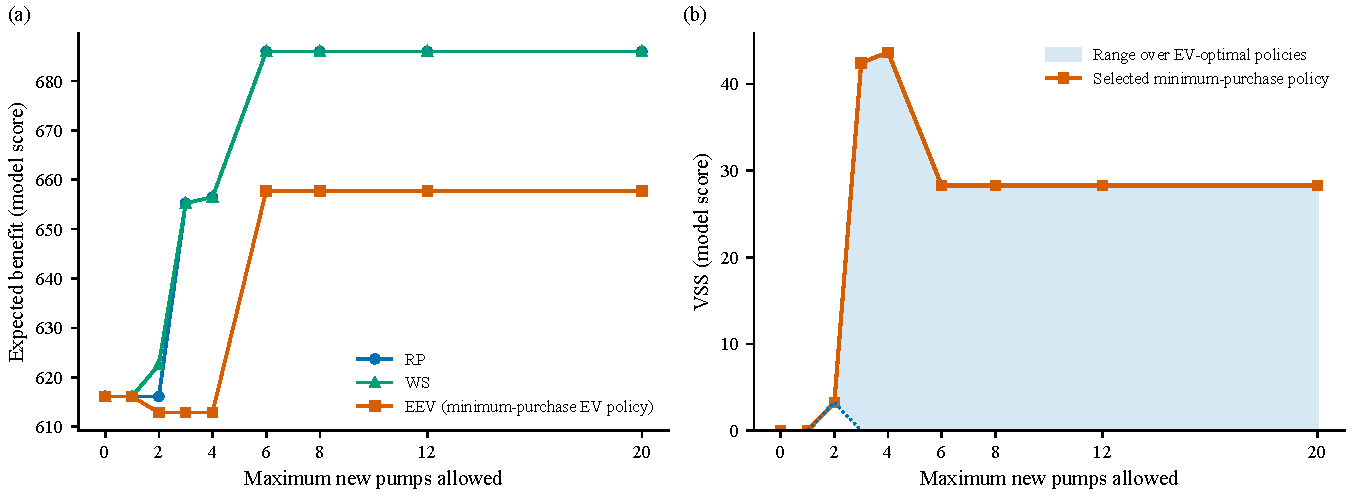
\includegraphics[width=\textwidth]{figures/fig01_inventory.pdf}
\caption{Procurement-limit sensitivity under zero initial stock, an approximate HKD1 million unit price and both-sector access. Original CU/score coefficients are held fixed. Left: RP, WS and EEV for the selected minimum-purchase EV policy. Right: selected-policy VSS and the range over all EV-optimal first-stage policies. Ten case specifications were audited, with 1,716 feasible first-stage policies enumerated in total. Shading is a policy range, not a confidence interval. Lines connect tested procurement limits.}
\label{fig:inventory}
\end{figure}

\begin{figure}[htbp]
\centering
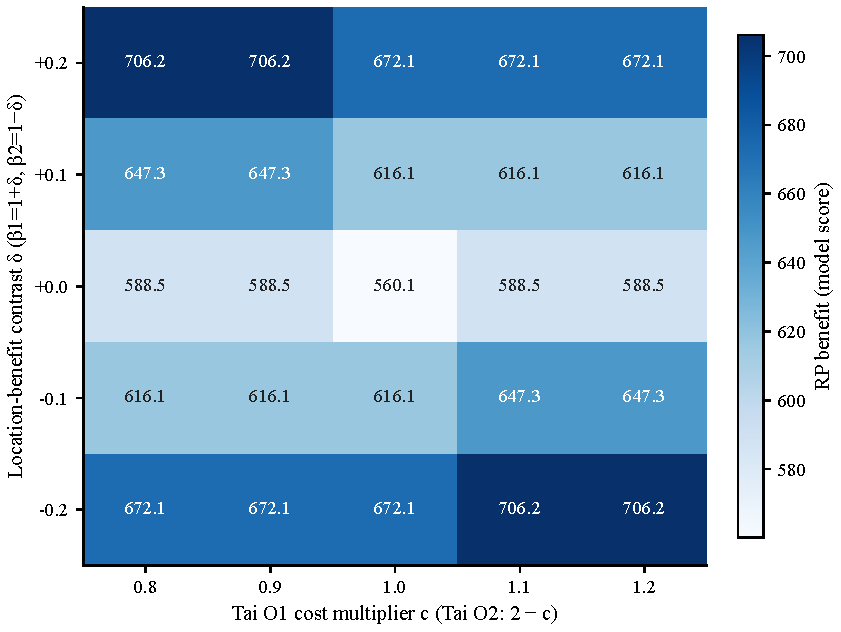
\includegraphics[width=0.7\textwidth]{figures/fig02_spatial.pdf}
\caption{Reoptimized RP for the 25 hypothetical spatial conditions, holding the inventory reference case fixed. Location modifiers are beta1=1+delta and beta2=1-delta; setup and deployment costs are multiplied by c in Tai O1 and 2-c in Tai O2. These perturbations are not estimated from the census population difference.}
\label{fig:spatial}
\end{figure}

\begin{figure}[htbp]
\centering
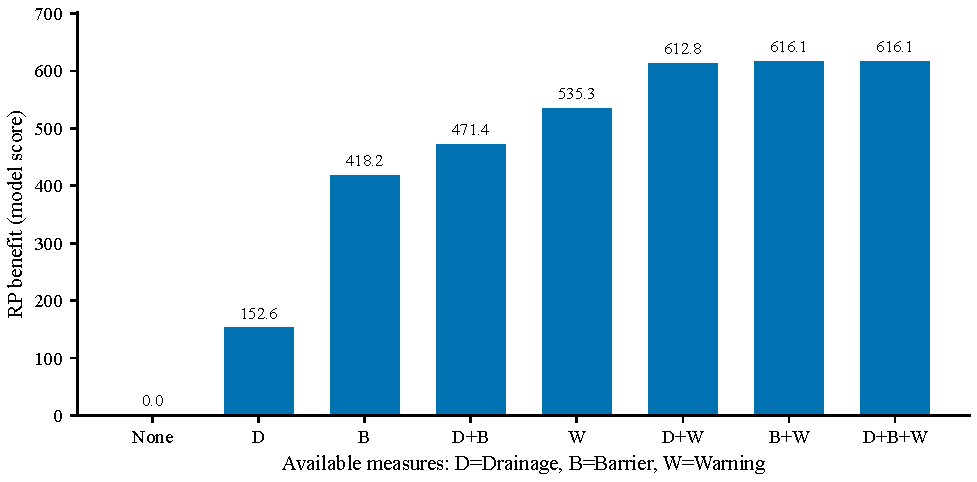
\includegraphics[width=0.85\textwidth]{figures/fig03_ablation.pdf}
\caption{RP across all eight subsets of Drainage, Barrier and Warning, with the same conditional inventory reference inputs. Each subset is reoptimized. The differences are model ablation effects, not causal estimates of real interventions.}
\label{fig:ablation}
\end{figure}

\begin{figure}[htbp]
\centering
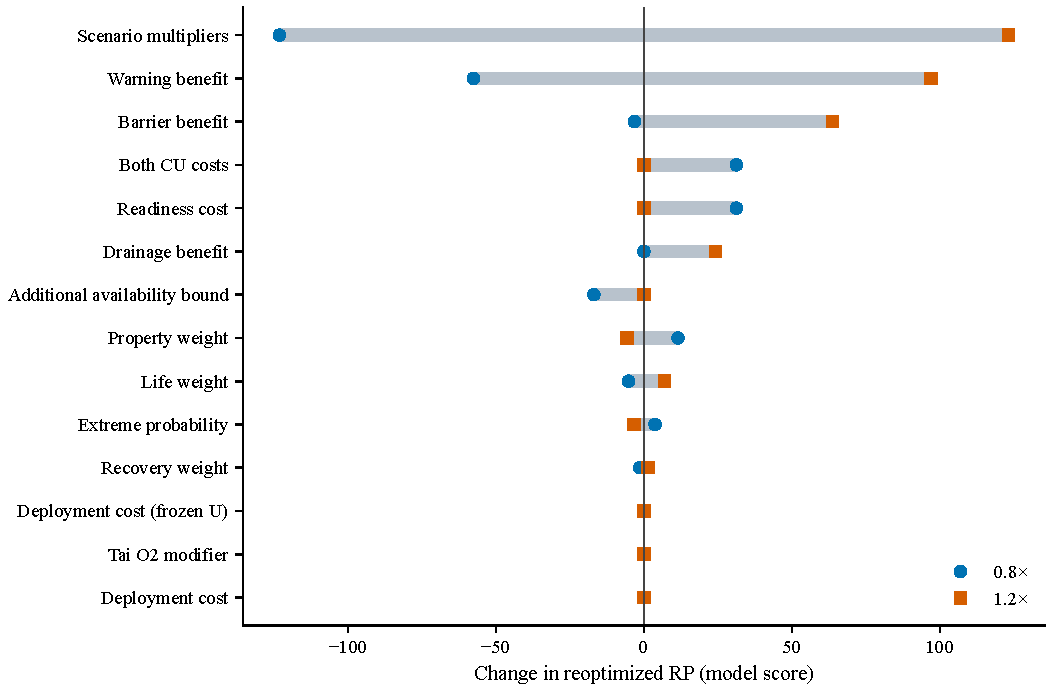
\includegraphics[width=0.9\textwidth]{figures/fig04_oat.pdf}
\caption{One-at-a-time endpoint effects relative to the inventory reference RP. Each of 14 factors has four tested levels; marks display its 0.8 and 1.2 endpoints, with the corresponding probabilities or weights renormalized where required. The fixed-old-U condition is an explicit control. Segments connect outcomes, not uncertainty intervals.}
\label{fig:oat}
\end{figure}

\begin{figure}[htbp]
\centering
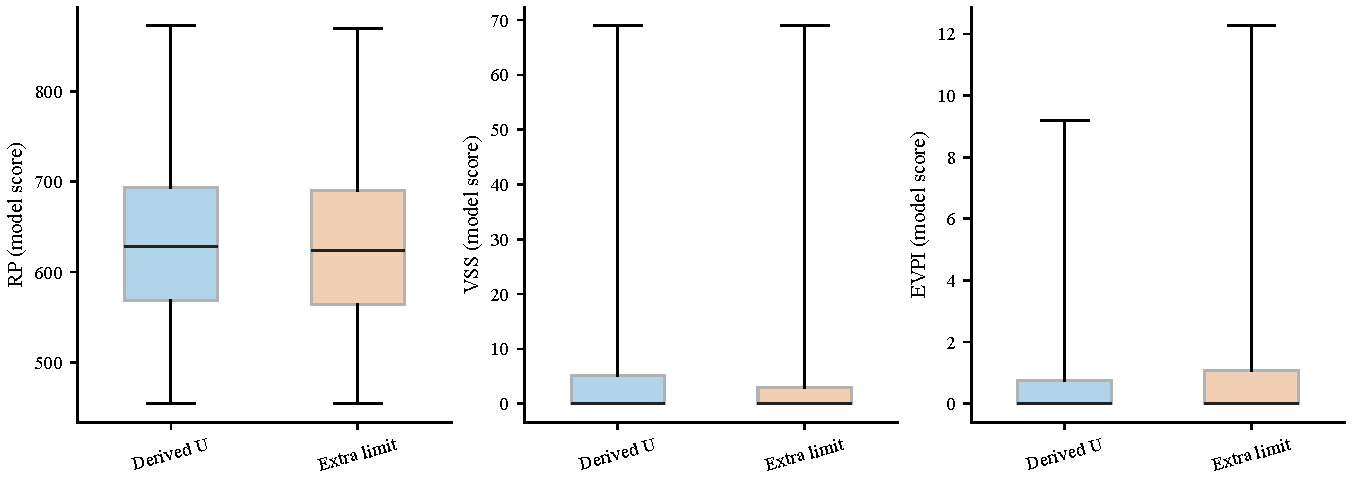
\includegraphics[width=\textwidth]{figures/fig05_uncertainty.pdf}
\caption{Outcome distributions over 200 paired hypothetical parameter draws per U convention, seed 20261103. Derived-U and extra-availability-limit conditions share each draw. Boxes show the interquartile range, lines the median and whiskers the minimum and maximum. VSS uses the stated minimum-procurement/readiness tie rule. These are parameter stress-test distributions, not confidence intervals or a common robust policy.}
\label{fig:uncertainty}
\end{figure}

\begin{figure}[htbp]
\centering
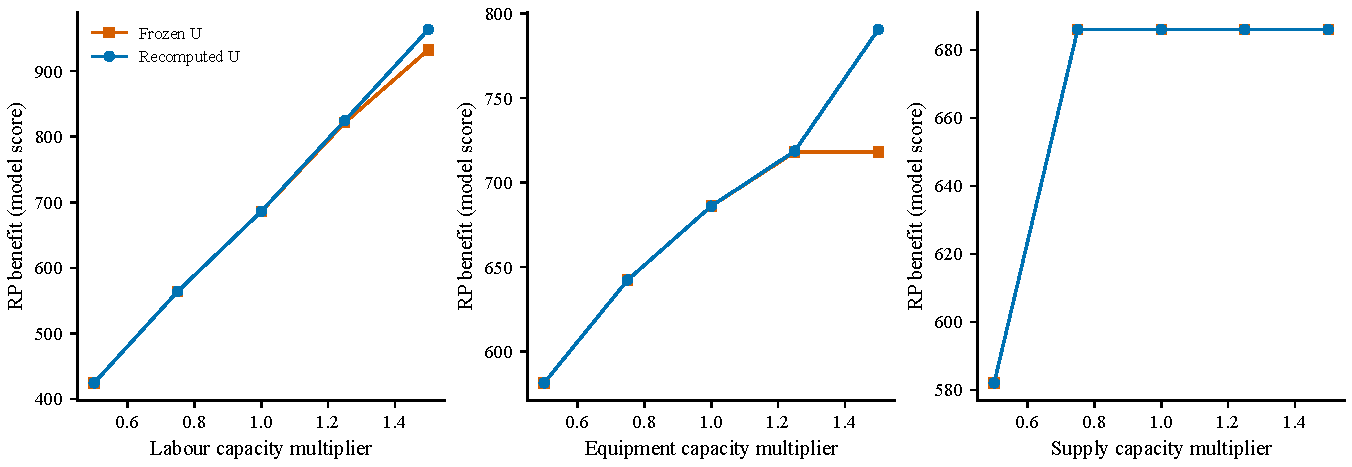
\includegraphics[width=\textwidth]{figures/fig06_bounds.pdf}
\caption{Legacy-model RP under frozen versus recomputed resource-derived linking bounds, five tested levels per resource. Costs, probabilities and benefit scores are unchanged. The comparison isolates a numerical bound correction; it does not include the new pump-stock constraint. Supply can change WS and EVPI even where its RP curves coincide; the accompanying correction table reports those outcomes.}
\label{fig:bounds}
\end{figure}
